今回使っているのは4輪走行ロボットである,
人間や昆虫の走行特徴に近似するため,超信地旋回が可能である.
tof距離センサーが赤外線の反射で距離を測るので,超音波より測る範囲が狭いが,
体積が小さく,精度が高くて,複数ロボットの場合,ロボット同士間の妨害も減少できる.
\begin{figure}[h]
    %\begin{minipage}{0.48\linewidth}
        \centering
        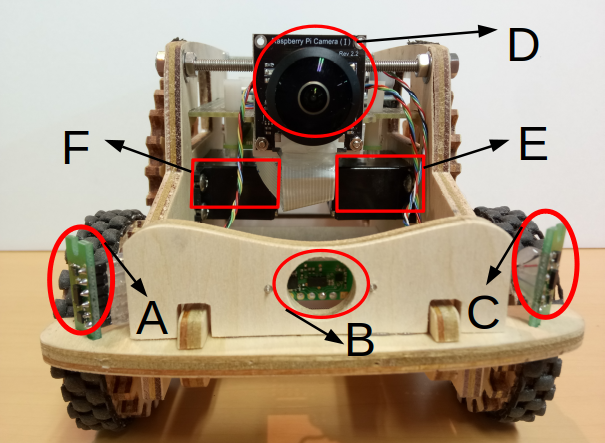
\includegraphics[width=0.9\linewidth]{robot1.jpg}
        \caption{正面図, A:右の距離センサー;
                 B:中央の距離センサー;
                 C:左の距離センサー;
                 D:カメラ(使っていない);
                 E:右モーター;
                 F:左モーター;
                 左右センサー角度:45\degree;
                 ロボット幅:13.5cm;ロボット長さ:20.2cm;ロボット高さ:12.2cm;
        }
    %\end{minipage}
    %\begin{minipage}{0.48\linewidth}
    %    \centering
    %    \includegraphics[width=0.9\linewidth]{robot2.jpg}
    %    \caption{俯瞰図}
    %\end{minipage}
\end{figure}
%\vspace{-6mm}
%\begin{figure}[h]
%        \centering
%        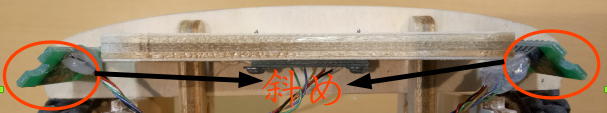
\includegraphics[width=1.0\linewidth]{robot4.jpg}
%        \caption{左右のセンサー角度表示}
%\end{figure}



